\section{Računska zahtevnost}
\label{sec:racunska_zahtevnost}
V tem poglavju podrobno analiziramo računsko zahtevnost algoritma v odvisnosti od velikosti množice nedominiranih točk $n = |\P|$ ter dimenzije problema $D$. Za lažjo analizo predpostavljamo, da je dimenzija $D$ konstanta, torej da lahko namesto $O(D)$ pišemo $O(1)$\footnote{Seveda pa dimenzije $D$ ne zanemarimo, ko ta nastopa v eksponentu.}. Predpostavka je smiselna, saj je računanje enostavnejših indikatorjev pri visokih dimenzijah zelo zamudno, tako da se v praksi le redko srečamo z več kot nekaj kriteriji. 

Najprej teoretično analiziramo časovno ter prostorsko zahtevnost, nato pa hitrost algoritma tudi testiramo za probleme dimenzij od 3 do 6, na množicah točk različnih velikost in oblik. Na koncu analiziramo še scenarij, kjer je algoritmu za množico paroma nedominiranih točk $\P$ danih več točk poizvedbe $\Q = \{\textbf{q}^1, \dots, \textbf{q}^m \}$ naenkrat. 

\subsection{Teoretična analiza časovne zahtevnosti}
\begin{izrek}
Algoritem ARRNO za računanje razdalje med nedominiranim območjem $N(\P)$ in točko poizvedbe $\textbf{q}$, ima časovno zahtevnost $O(n \log n)$ za $D=3$ in $O(n^{D-1})$ za $D \geq 4$, kjer je $n = |\P|$ in $D$ dimenzija prostora.
\end{izrek}
Časovna zahtevnost algoritma ARRNO je sestavljena iz časovne zahtevnosti računanja množice vpetih točk $\V$ ter časovne zahtevnosti iskanja razdalje do najbližjega stožca, ki ga razpenjajo vpete točke. Naj bo število vpetih točk enako $v$. Potem očitno poiščemo najbližji stožec v $O(v)$. Ker pa smo pri konstrukciji vpetih točk gotovo konstruirali vsako izmed njih, je časovna zahtevnost iskanja vpetih točk vsaj $O(v)$. Torej zadošča izračunati časovno zahtevnost algoritma \Call{Vpete točke}{$\P$}. Vseeno pa najprej pokažimo, kolikšno je maksimalno število vpetih točk $\V$, glede na dimenzijo problema. 

\begin{trditev}
\label{sec:st_vpetih_tock}
Za dimenzijo $D=2, 3$ je število vpetih točk $O(n)$, kjer je $n = |\P|$. Za $D=4$ je število vpetih točk $O(n^2)$ in obstajajo take množice točk $\P$, za katere je število vpetih točk $\Omega(n^2)$. Za $D > 4$ je število vpetih točk $O(n^{D-2})$.
\end{trditev}

\begin{dokaz}
V algoritmu \Call{Vpete točke 3D}{$\P$}, za računanje vpetih točk v treh dimenzijah, na vsakem koraku zanke (algoritem \ref{alg:vpete_tocke_3d}, vrstice 6--16) v stanje $\sv$ dodamo največ dve točki. Skupaj s točko $(0, 0)$, ki je v množici $\sv$ od začetka, torej v $\sv$ dodamo največ $2n + 1$ točk. Ker vpete točke računamo tako, da jih postopoma odstranjujemo iz $\sv$, bo tudi vpetih točk največ $2n + 1$. 
    
Kadar rešujemo problem v štirih dimenzijah  (algoritem \ref{alg:vpete_tocke}, vrstica 14), $n$-krat dodamo vpete točke tridimenzionalnega podproblema. Torej je vpetih točk v štirih dimenzijah največ
\[
1 + \sum_{i=1}^n 2i + 1 = (n + 1) + 2 \sum_{i=1}^n i = (n + 1) + n(n + 1) = (n + 1)^2 = O(n^2).
\] 
Da je kvadratično število vpetih točk v štirih dimenzijah res tesna meja, pokažemo na primeru. Sestavimo tak primer, kjer pri dodajanju prve polovice točk vsakič dobimo konstantno število vpetih točk, pri dodajanju druge polovice točk, pa vsakič linearno število novih vpetih točk. Tak primer je na primer množica točk
\[
\left \{(i + 1, \frac{n}{2} - i, n - i, n - i) \mid  i = 0, 1, \dots \frac{n}{2} - 1 \right \},
\]
za prvo polovico točk, ter 
\[
\left \{(n - i, n - i, i + 1, \frac{n}{2} - i) \mid  i = 0, 1, \dots \frac{n}{2} - 1 \right \},
\]
za drugo polovico točk. Na sliki~\ref{fig:example4d} vidimo vizualizacijo tridimenzionalnega stanja $\sp$ za primer $n = 6$ po dodajanju prvih treh, štirih, petih in šestih točk. 

\begin{figure}[ht]
    \centering
    \begin{subfigure}{0.495\textwidth}
        \centering
        \begin{tikzpicture}
    % lines:
    \draw (-0.9239,2.2346) -- (-1.3858,2.426);
    \draw (-1.3858,2.426) -- (0.0,3.0);
    \draw (-1.3858,2.426) -- (-1.3858,-0.574);
    \draw (-0.9239,2.2346) -- (0.4619,2.8087);
    \draw (0.4619,2.8087) -- (0.0,3.0);
    \draw (0.4619,2.8087) -- (0.4619,2.3087);
    \draw (-0.9239,2.2346) -- (-0.9239,-0.7654);
    \draw (-0.9239,-0.7654) -- (-1.3858,-0.574);
    \draw (-0.9239,-0.7654) -- (-0.4619,-0.574);
    \draw (0.0,1.7346) -- (-0.4619,1.926);
    \draw (-0.4619,1.926) -- (0.4619,2.3087);
    \draw (-0.4619,1.926) -- (-0.4619,-0.574);
    \draw (0.0,1.7346) -- (0.9239,2.1173);
    \draw (0.9239,2.1173) -- (0.4619,2.3087);
    \draw (0.9239,2.1173) -- (0.9239,1.6173);
    \draw (0.0,1.7346) -- (0.0,-0.7654);
    \draw (0.0,-0.7654) -- (-0.4619,-0.574);
    \draw (0.0,-0.7654) -- (0.4619,-0.574);
    \draw (0.9239,1.2346) -- (0.4619,1.426);
    \draw (0.4619,1.426) -- (0.9239,1.6173);
    \draw (0.4619,1.426) -- (0.4619,-0.574);
    \draw (0.9239,1.2346) -- (1.3858,1.426);
    \draw (1.3858,1.426) -- (0.9239,1.6173);
    \draw (1.3858,1.426) -- (1.3858,-0.574);
    \draw (0.9239,1.2346) -- (0.9239,-0.7654);
    \draw (0.9239,-0.7654) -- (0.4619,-0.574);
    \draw (0.9239,-0.7654) -- (1.3858,-0.574);
    % points:
    \fill[black] (-0.9238795325112866,2.2346331352698203) circle (2pt) ;
    \fill[black] (0.0,1.7346331352698203) circle (2pt) ;
    \fill[black] (0.9238795325112866,1.2346331352698203) circle (2pt) ;
    % kink points:
    \fill[nodecol] (0.9238795325112867,1.6173165676349102) circle (2pt) ;
    \fill[nodecol] (0.46193976625564337,-0.5740251485476346) circle (2pt) ;
    \fill[nodecol] (1.38581929876693,-0.5740251485476346) circle (2pt) ;
    % axes:
    \draw[->] (1.3858,-0.574) -- (3.2336,-1.3394) node[midway, below] {\( f_1 \)};
    \draw[->] (-1.3858,-0.574) -- (-3.2336,-1.3394) node[midway, below] {\( f_2 \)};
    \draw[->] (0.0,3.0) -- (0.0,3.5) node[midway, right] {\( f_3 \)};
\end{tikzpicture}
        \caption{Stanje po dodajanju tretje točke.}
        \label{example4d_1}
    \end{subfigure}
    \hfill
    \begin{subfigure}{0.495\textwidth}
        \centering
        \begin{tikzpicture}
    % lines:
    \draw (-0.9239,2.2346) -- (-1.3858,2.426);
    \draw (-1.3858,2.426) -- (0.0,3.0);
    \draw (-1.3858,2.426) -- (-1.3858,-0.074);
    \draw (-0.9239,2.2346) -- (0.4619,2.8087);
    \draw (0.4619,2.8087) -- (0.0,3.0);
    \draw (0.4619,2.8087) -- (0.4619,2.3087);
    \draw (-0.9239,2.2346) -- (-0.9239,-0.2654);
    \draw (-0.9239,-0.2654) -- (-1.3858,-0.074);
    \draw (-0.9239,-0.2654) -- (-0.4619,-0.074);
    \draw (0.0,1.7346) -- (-0.4619,1.926);
    \draw (-0.4619,1.926) -- (0.4619,2.3087);
    \draw (-0.4619,1.926) -- (-0.4619,-0.074);
    \draw (0.0,1.7346) -- (0.9239,2.1173);
    \draw (0.9239,2.1173) -- (0.4619,2.3087);
    \draw (0.9239,2.1173) -- (0.9239,1.6173);
    \draw (0.0,1.7346) -- (0.0,-0.2654);
    \draw (0.0,-0.2654) -- (-0.4619,-0.074);
    \draw (0.0,-0.2654) -- (0.4619,-0.074);
    \draw (0.9239,1.2346) -- (0.4619,1.426);
    \draw (0.4619,1.426) -- (0.9239,1.6173);
    \draw (0.4619,1.426) -- (0.4619,-0.074);
    \draw (0.9239,1.2346) -- (1.3858,1.426);
    \draw (1.3858,1.426) -- (0.9239,1.6173);
    \draw (1.3858,1.426) -- (1.3858,-0.074);
    \draw (0.9239,1.2346) -- (0.9239,-0.2654);
    \draw (0.9239,-0.2654) -- (0.4619,-0.074);
    \draw (0.9239,-0.2654) -- (1.3858,-0.074);
    \draw (0.0,-1.7961) -- (-2.7716,-0.6481);
    \draw (-2.7716,-0.6481) -- (-1.3858,-0.074);
    \draw (-2.7716,-0.6481) -- (-2.7716,-1.1481);
    \draw (0.0,-1.7961) -- (2.7716,-0.6481);
    \draw (2.7716,-0.6481) -- (1.3858,-0.074);
    \draw (2.7716,-0.6481) -- (2.7716,-1.1481);
    \draw (0.0,-1.7961) -- (0.0,-2.2961);
    \draw (0.0,-2.2961) -- (-2.7716,-1.1481);
    \draw (0.0,-2.2961) -- (2.7716,-1.1481);
    % points:
    \fill[black] (-0.9238795325112866,2.2346331352698203) circle (2pt) ;
    \fill[black] (0.0,1.7346331352698203) circle (2pt) ;
    \fill[black] (0.9238795325112866,1.2346331352698203) circle (2pt) ;
    \fill[black] (0.0,-1.7961005941905386) circle (2pt) ;
    % kink points:
    \fill[nodecol] (-1.38581929876693,-0.07402514854763464) circle (2pt) ;
    \fill[nodecol] (-0.46193976625564337,-0.07402514854763464) circle (2pt) ;
    \fill[nodecol] (0.46193976625564337,-0.07402514854763464) circle (2pt) ;
    \fill[nodecol] (1.38581929876693,-0.07402514854763464) circle (2pt) ;
    \fill[nodecol] (-2.77163859753386,-1.1480502970952693) circle (2pt) ;
    \fill[nodecol] (2.77163859753386,-1.1480502970952693) circle (2pt) ;
    % axes:
    \draw[->] (2.7716,-1.1481) -- (3.2336,-1.3394) node[midway, below] {\( f_1 \)};
    \draw[->] (-2.7716,-1.1481) -- (-3.2336,-1.3394) node[midway, below] {\( f_2 \)};
    \draw[->] (0.0,3.0) -- (0.0,3.5) node[midway, right] {\( f_3 \)};
\end{tikzpicture}
        \caption{Stanje po dodajanju četrte točke.}
        \label{example4d_2}
    \end{subfigure}

    \vspace{0.5cm}

    \begin{subfigure}{0.495\textwidth}
        \centering
        \begin{tikzpicture}
    % lines:
    \draw (-0.9239,2.2346) -- (-1.3858,2.426);
    \draw (-1.3858,2.426) -- (0.0,3.0);
    \draw (-1.3858,2.426) -- (-1.3858,0.426);
    \draw (-0.9239,2.2346) -- (0.4619,2.8087);
    \draw (0.4619,2.8087) -- (0.0,3.0);
    \draw (0.4619,2.8087) -- (0.4619,2.3087);
    \draw (-0.9239,2.2346) -- (-0.9239,0.2346);
    \draw (-0.9239,0.2346) -- (-1.3858,0.426);
    \draw (-0.9239,0.2346) -- (-0.4619,0.426);
    \draw (0.0,1.7346) -- (-0.4619,1.926);
    \draw (-0.4619,1.926) -- (0.4619,2.3087);
    \draw (-0.4619,1.926) -- (-0.4619,0.426);
    \draw (0.0,1.7346) -- (0.9239,2.1173);
    \draw (0.9239,2.1173) -- (0.4619,2.3087);
    \draw (0.9239,2.1173) -- (0.9239,1.6173);
    \draw (0.0,1.7346) -- (0.0,0.2346);
    \draw (0.0,0.2346) -- (-0.4619,0.426);
    \draw (0.0,0.2346) -- (0.4619,0.426);
    \draw (0.9239,1.2346) -- (0.4619,1.426);
    \draw (0.4619,1.426) -- (0.9239,1.6173);
    \draw (0.4619,1.426) -- (0.4619,0.426);
    \draw (0.9239,1.2346) -- (1.3858,1.426);
    \draw (1.3858,1.426) -- (0.9239,1.6173);
    \draw (1.3858,1.426) -- (1.3858,0.426);
    \draw (0.9239,1.2346) -- (0.9239,0.2346);
    \draw (0.9239,0.2346) -- (0.4619,0.426);
    \draw (0.9239,0.2346) -- (1.3858,0.426);
    \draw (0.0,-1.7961) -- (-2.7716,-0.6481);
    \draw (-2.7716,-0.6481) -- (-2.3097,-0.4567);
    \draw (-2.7716,-0.6481) -- (-2.7716,-1.1481);
    \draw (0.0,-1.7961) -- (2.7716,-0.6481);
    \draw (2.7716,-0.6481) -- (2.3097,-0.4567);
    \draw (2.7716,-0.6481) -- (2.7716,-1.1481);
    \draw (0.0,-1.7961) -- (0.0,-2.2961);
    \draw (0.0,-2.2961) -- (-2.7716,-1.1481);
    \draw (0.0,-2.2961) -- (2.7716,-1.1481);
    \draw (0.0,-0.9134) -- (-2.3097,0.0433);
    \draw (-2.3097,0.0433) -- (-1.3858,0.426);
    \draw (-2.3097,0.0433) -- (-2.3097,-0.4567);
    \draw (0.0,-0.9134) -- (2.3097,0.0433);
    \draw (2.3097,0.0433) -- (1.3858,0.426);
    \draw (2.3097,0.0433) -- (2.3097,-0.4567);
    \draw (0.0,-0.9134) -- (0.0,-1.4134);
    \draw (0.0,-1.4134) -- (-2.3097,-0.4567);
    \draw (0.0,-1.4134) -- (2.3097,-0.4567);
    % points:
    \fill[black] (-0.9238795325112866,2.2346331352698203) circle (2pt) ;
    \fill[black] (0.0,1.7346331352698203) circle (2pt) ;
    \fill[black] (0.9238795325112866,1.2346331352698203) circle (2pt) ;
    \fill[black] (0.0,-1.7961005941905386) circle (2pt) ;
    \fill[black] (0.0,-0.913417161825449) circle (2pt) ;
    % kink points:
    \fill[nodecol] (-1.38581929876693,0.42597485145236536) circle (2pt) ;
    \fill[nodecol] (-0.46193976625564337,0.42597485145236536) circle (2pt) ;
    \fill[nodecol] (0.46193976625564337,0.42597485145236536) circle (2pt) ;
    \fill[nodecol] (1.38581929876693,0.42597485145236536) circle (2pt) ;
    \fill[nodecol] (-2.309698831278217,-0.4567085809127245) circle (2pt) ;
    \fill[nodecol] (2.309698831278217,-0.4567085809127245) circle (2pt) ;
    % axes:
    \draw[->] (2.7716,-1.1481) -- (3.2336,-1.3394) node[midway, below] {\( f_1 \)};
    \draw[->] (-2.7716,-1.1481) -- (-3.2336,-1.3394) node[midway, below] {\( f_2 \)};
    \draw[->] (0.0,3.0) -- (0.0,3.5) node[midway, right] {\( f_3 \)};
\end{tikzpicture}
        \caption{Stanje po dodajanju pete točke.}
        \label{example4d_3}
    \end{subfigure}
    \hfill
    \begin{subfigure}{0.495\textwidth}
        \centering
        \input{tikz_images/example4d_4}
        \caption{Stanje po dodajanju šeste točke.}
        \label{example4d_4}
    \end{subfigure}

    \caption{Vizualizacija stanja $\sp$ po dodajanju točk iz $\P$. S črno barvo so označene točke v $\sp$, z oranžno barvo pa novonastale vpete točke pri dodajanju zadnje točke v $\sp$. Pri dodajanju prvih $\frac{n}{2}$ točk vsakič nastanejo tri nove vpete točke, kot vidimo na sliki~\ref{example4d_1}. Pri dodajanju druge polovice točk, pa vsakič nastane $(\frac{n}{2} + 1) + 2$ novih vpetih točk, kot vidimo na slikah~\ref{example4d_2},~\ref{example4d_3} in~\ref{example4d_4}.}
    \label{fig:example4d}
\end{figure}

Podobno kot za število vpetih točk v štirih dimenzijah, lahko tudi za dimenzije $D > 4$ pokažemo, da je vpetih točk največ $O(n^{D-2})$. Ne vemo pa, ali je ta zgornja meja tesna. Glede na to, da je število vpetih točk v dveh in treh dimenzijah linearno, bi bilo prav tako mogoče, da je vpetih točk $O(n^{\lfloor \frac{D}{2} \rfloor})$. Taka meja se pojavi pri problemu Kleejeve mere~\cite{Bringmann}, torej računanja volumna unije kvadrov vzporednih z koordinatnimi osmi.
\end{dokaz}

\subsubsection{Časovna zahtevnost v treh dimenzijah} 
Najprej si oglejmo algoritem \Call{Vpete točke 3d}{$\P$} (algoritem \ref{alg:vpete_tocke_3d}).
Za inicializacijo struktur $\V$, $\sp$, $\sv$ in $h$ porabimo konstanten čas. Množico $\V$ implementiramo kot seznam, stanji $\sp$ in $\sv$ kot urejen seznam, ki podpira dodajanje in iskanje v logaritemskem času~\cite{sortedcontainers}, $h$ pa kot zgoščevalno funkcijo.

Nato v zanki (vrstice 6--16) $n$-krat izvedemo več ukazov. Funkcija \Call{Odstrani dominirane}{$\sv, \overline{\textbf{p}}$} z bisekcijo poišče prvi ter zadnji dominiran element, nato pa ju odstrani in vrne, skupaj z vsemi elementi seznama vmes. Torej je zahtevnost funkcije enaka $O(\log|\sv| + k)$, kjer je $k$ število dominiranih točk v $\sv$. Ker je vsaka točka iz množice $\sv$ odstranjena le enkrat in bo vseh vpetih točk največ $O(n)$, bo po $n$ iteracijah skupna časovna zahtevnost funkcije enaka $O(n \log n)$. 
Podobno se tudi notranjost naslednje zanke (vrstice 9--10), skozi vse iteracije zunanje zanke, izvede le $O(n)$-krat. Znotraj zanke so vse operacije konstantne, torej je skupna časovna zahtevnost vrstic 8--10, skozi celotno delovanje algoritma, enaka $O(n)$. 
V vrstici 11 stanju $\sp$ dodamo novo točko, kar naredimo v $O(\log|\sp|) = O(\log n)$, saj je stanje $\sp$ vedno manjše od števila točk $n$. 
Prav tako v logaritemskem času izračunamo tudi novi vpeti točki, za izračun potrebujemo le indeks elementa $\overline{\textbf{p}}$ v množici $\sp$, nato pa točki izračunamo s pomočjo sosednjih elementov v seznamu. 
Ker je iskanje in nastavljanje elementa v zgoščevalni funkciji v povprečju konstantno, se tudi vrstice 13--15 izvedejo v konstantnem času, dodajanje v stanje $\sv$ pa zopet porabi $O(\log n)$. Torej za celotno zanko for (vrstice 6--16) algoritem porabi $O(n \log n)$ časa. 
Na koncu le še poskrbimo za preostale točke v $\sv$, za katere pa smo že pokazali, da jih je največ $O(n)$. 

Torej je skupna časovna zahtevnost algoritma za iskanje vpetih točk v treh dimenzijah (ter potem tudi algoritma ARRNO v treh dimenzijah) $O(n \log n)$.

\subsubsection{Časovna zahtevnost v višjih dimenzijah}
Naj bo $T(n, D)$ čas, ki ga porabi algoritem za vhodno množico $|\P| = n$ in dimenzijo $D$. Pokazali smo že, da je $T(n, 3) = O(n \log n)$, zdaj pa bi radi izračunali $T(n, D)$ še za poljubno dimenzijo $D > 3$.

Tudi v višjih dimenzijah za inicializacijo stanj potrebujemo konstanten čas, časovno najbolj zahtevne operacije, pa se zgodijo znotraj glavne zanke algoritma \ref{alg:vpete_tocke}. Funkcijo \Call{Odstrani Dominirane}{$\sv, \overline{\textbf{p}}$}, kličemo $n$ krat in potrebuje linearno časovno zahtevnost v odvisnosti od števila točk v $\sv$. Ker je število točk v $\sv$ omejeno z $O(n^{D-2})$, je časovna zahtevnost funkcije v najslabšem primeru $O(n^{D-1})$. Po enakem razmisleku kot v algoritmu treh dimenzij, algoritem za vrstice 10--12 porabi $O(n^{D-2})$ časa. Za dodajanje točke $\overline{\textbf{p}}$ v stanje $\sp$, skupaj z odstranjevanjem dominiranih točk pa je na vsakem koraku potrebno $O(n)$ časa, torej skupaj $O(n^2)$. Računanje novih vpetih točk in dodajanje točk v zgoščevalno funkcijo $h$ v vrsticah 14--17, pa ima znotraj vsake ponovitve časovno zahtevnost $T(n, D-1)$. Za dodajanje preostalih točk iz $\sv$ v $\V(\P)$ pa je potrebno največ $O(n^{D-2})$ časa, kolikor je možnih točk v $\sv$. Torej velja
\[
T(n, D) = O(n^{D-1}) + n T(n, D-1).
\]
Za $D = 4$ torej velja
\[
T(n, 4) = O(n^{3}) + O(n^2 \log n) = O(n^3),
\]
za splošen $D \geq 4$ pa
\[
T(n, D) = O(n^{D-1}).
\]

\subsection{Analiza prostorske zahtevnosti}
Za analizo prostorske zahtevnosti algoritma, spremljamo strukture $\P$ $\V$, $\overline{\V}$, $\sp$, $\sv$ in $h$ tekom algoritma. Vse ostale spremenljivke zasedajo konstantno veliko prostora. Vhodna množica $\P$ je velikosti $O(n)$, kakor tudi stanje $\sp$, ki se inicializira prazno, na koncu pa ima največ $O(n)$ točk. Za izhodno množico vpetih točk smo v trditvi~\ref{sec:st_vpetih_tock} pokazali da vsebuje največ $O(n^{D-2})$ točk, množica $\overline{\V}$ pa $O(n^{D-3})$ točk, saj predstavlja vpete točke problema v nižji dimenziji. Enako kot $\V$ potrebujeta tudi stanje $\sv$ in zgoščevalna funkcija $h$ največ $O(n^{D-2})$ prostora. 

Upoštevati je potrebno tudi prostor, ki ga zasede tudi klicanje rekurzivne funkcije. Znotraj funkcije sicer $n$ krat rekurzivno kličemo funkcijo z nižjo dimenzijo, vendar se hkrati izvaja vedno največ en klic funkcije za vsako dimenzijo $D \geq 3$. Torej je skupna prostorska zahtevnost enaka
\[
\sum_{i=3}^D O(n^{i-2}) = O(n^{D-2}).
\]

\subsection{Eksperimentalna analiza časovne zahtevnosti}
Za ovrednotenje hitrosti algoritma ARRNO izvedemo serijo poskusov pri dimenzijah problema 3, 4, 5 in 6. Testiranje algoritma pri višjih dimenzijah problema je zaradi eksponentne časovne zahtevnosti dolgotrajno, prav tako pa za to tudi ni prave motivacije, saj se z večkriterijsko optimizacijo s tolikšnim številom kriterijev v praksi srečamo redko. 

Testne instance ustvarimo tako, da čim bolj posnemajo scenarij večkriterijske optimizacije, kjer skozi proces optimizacije dobivamo množico paroma nedominiranih točk, ki ji rečemo fronta. Dva primera takih front, ki se pogosto pojavita v raziskavah in se enostavno generalizirata na poljubno število dimenzij sta sferična ter linearna fronta~\cite{Tusar15tevc}. Prav tako pa ustvarimo tudi poseben primer fronte, za katero pričakujemo, da je za algoritem najbolj časovno zahtevna. 

\subsubsection{Linearna fronta}
Linearna fronta je sestavljena iz točk, ki ležijo na hiperravnini v pozitivnem delu koordinatnega sistema in predstavlja primer večkriterijskega problema z linearnim kompromisom med kriteriji. Primera front v dveh in treh dimenzijah vidimo na sliki~\ref{fig:linear_front}.

\begin{figure}[th]
    \centering
    \begin{subfigure}{0.45\textwidth}
        \centering
        \begin{tikzpicture}
  \begin{axis}[
    xlabel={$f_1$},
    ylabel={$f_2$},
    xmin=0, xmax=3.5,
    ymin=0, ymax=3.5,
    width=6cm,
    height=6cm,
    enlargelimits=true,
    axis lines=middle,
    ticks=none
  ]
    \addplot[
      only marks,
      mark=*,
      Greens-I
    ] table [x=x, y=y, col sep=comma] {csv/points_linear_2D.csv};

  \addplot[Greens-F, line width=2pt] coordinates {(0,3) (3,0)};
  
  \end{axis}
\end{tikzpicture}

        \caption{Primer linearne fronte z 20 točkami v dveh dimenzijah.}
        \label{fig:front_linear_2d}
    \end{subfigure}
    \hfill
    \begin{subfigure}{0.45\textwidth}
        \centering
        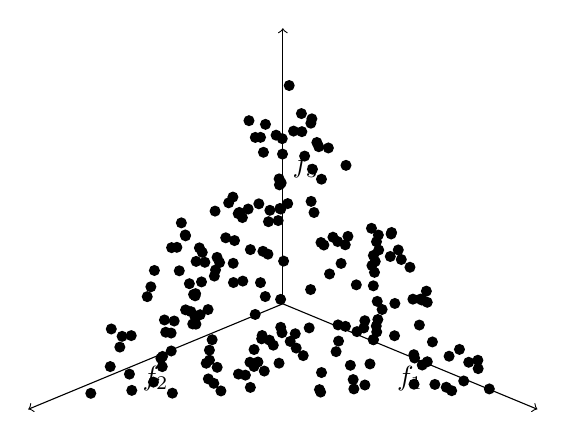
\begin{tikzpicture}
    % lines:
    % points:
    \fill[black] (0.9021195157091322,-1.0810397367966744) circle (2pt) node[below left] {\(  \)};
    \fill[black] (2.6221823312340318,-1.0809484483225305) circle (2pt) node[below left] {\(  \)};
    \fill[black] (1.1256565705599428,0.958895773509134) circle (2pt) node[below left] {\(  \)};
    \fill[black] (2.476711115777088,-0.7166943740610576) circle (2pt) node[below left] {\(  \)};
    \fill[black] (-1.6310821800211837,0.42354247730178773) circle (2pt) node[below left] {\(  \)};
    \fill[black] (1.0279372141835572,-0.306301537213135) circle (2pt) node[below left] {\(  \)};
    \fill[black] (0.25880308665291407,-0.6576996491681348) circle (2pt) node[below left] {\(  \)};
    \fill[black] (-1.2358717329771969,0.863285832855884) circle (2pt) node[below left] {\(  \)};
    \fill[black] (-0.03760532061931643,1.2104441188645239) circle (2pt) node[below left] {\(  \)};
    \fill[black] (-0.47546362621536487,-0.9057782803309733) circle (2pt) node[below left] {\(  \)};
    \fill[black] (0.37625770552387683,1.7095817019652415) circle (2pt) node[below left] {\(  \)};
    \fill[black] (-1.1080895725391637,0.12916218409637126) circle (2pt) node[below left] {\(  \)};
    \fill[black] (1.163773036033838,0.3994805543876424) circle (2pt) node[below left] {\(  \)};
    \fill[black] (-0.36655881562829284,-0.795851449492381) circle (2pt) node[below left] {\(  \)};
    \fill[black] (-0.8354800214675406,0.5899811817588534) circle (2pt) node[below left] {\(  \)};
    \fill[black] (-0.3651699190593616,-0.5805157677055917) circle (2pt) node[below left] {\(  \)};
    \fill[black] (-0.269068188527702,-0.44439713919340373) circle (2pt) node[below left] {\(  \)};
    \fill[black] (0.3527212984247433,0.18095860779843242) circle (2pt) node[below left] {\(  \)};
    \fill[black] (-1.1136501576651119,0.10118196510908861) circle (2pt) node[below left] {\(  \)};
    \fill[black] (-0.9323167426407631,-0.5884663083224728) circle (2pt) node[below left] {\(  \)};
    \fill[black] (1.4185918633858157,-0.40542620369525306) circle (2pt) node[below left] {\(  \)};
    \fill[black] (-0.16468076798276465,1.1875135273883561) circle (2pt) node[below left] {\(  \)};
    \fill[black] (-0.9461566062146752,-0.953684731395585) circle (2pt) node[below left] {\(  \)};
    \fill[black] (-0.4300009850306819,2.325883977421264) circle (2pt) node[below left] {\(  \)};
    \fill[black] (1.1316989450977644,0.486321601602169) circle (2pt) node[below left] {\(  \)};
    \fill[black] (-0.047156502194816485,1.5865797163789863) circle (2pt) node[below left] {\(  \)};
    \fill[black] (-0.08556659961075125,2.141785342868388) circle (2pt) node[below left] {\(  \)};
    \fill[black] (-1.1440929859374342,-0.2558613902881015) circle (2pt) node[below left] {\(  \)};
    \fill[black] (0.43193524811940615,2.048867070634025) circle (2pt) node[below left] {\(  \)};
    \fill[black] (1.217298718292569,0.6836625125747742) circle (2pt) node[below left] {\(  \)};
    \fill[black] (1.1500014617669112,0.6138487835565276) circle (2pt) node[below left] {\(  \)};
    \fill[black] (-2.041266114610905,-0.41295478953896314) circle (2pt) node[below left] {\(  \)};
    \fill[black] (-0.949730517565904,-0.0729133546054288) circle (2pt) node[below left] {\(  \)};
    \fill[black] (-0.9314354592829076,-0.7148833681793494) circle (2pt) node[below left] {\(  \)};
    \fill[black] (-0.6135020496582938,0.8032371414444686) circle (2pt) node[below left] {\(  \)};
    \fill[black] (-0.004225822933933976,1.901783825498005) circle (2pt) node[below left] {\(  \)};
    \fill[black] (1.1867950297403032,-0.2823529384521237) circle (2pt) node[below left] {\(  \)};
    \fill[black] (0.7954201494980967,-0.28611144981659065) circle (2pt) node[below left] {\(  \)};
    \fill[black] (0.009903835646007053,0.5423169109202521) circle (2pt) node[below left] {\(  \)};
    \fill[black] (0.09361156271610871,-0.4776927096141246) circle (2pt) node[below left] {\(  \)};
    \fill[black] (-0.28330126527362554,2.114176783481734) circle (2pt) node[below left] {\(  \)};
    \fill[black] (-1.9481909950961886,-0.8930065344623515) circle (2pt) node[below left] {\(  \)};
    \fill[black] (1.6734022180696178,-0.6882670343519766) circle (2pt) node[below left] {\(  \)};
    \fill[black] (-0.5522870448167116,1.1607182197755357) circle (2pt) node[below left] {\(  \)};
    \fill[black] (1.4226967746113395,0.004655687417944199) circle (2pt) node[below left] {\(  \)};
    \fill[black] (-0.6878228215069788,1.2826678865108398) circle (2pt) node[below left] {\(  \)};
    \fill[black] (0.792779886654227,0.7494365711832691) circle (2pt) node[below left] {\(  \)};
    \fill[black] (0.1697369993627016,-0.5619186970595387) circle (2pt) node[below left] {\(  \)};
    \fill[black] (1.6144329077787238,0.4642769247879647) circle (2pt) node[below left] {\(  \)};
    \fill[black] (-1.1013937938076226,0.5387273684915526) circle (2pt) node[below left] {\(  \)};
    \fill[black] (1.748389986800012,0.060218958517676335) circle (2pt) node[below left] {\(  \)};
    \fill[black] (0.4803078475862319,-1.1211157640962197) circle (2pt) node[below left] {\(  \)};
    \fill[black] (-1.4028894520880464,-1.1348498574107884) circle (2pt) node[below left] {\(  \)};
    \fill[black] (1.375303147502073,0.8869027257816798) circle (2pt) node[below left] {\(  \)};
    \fill[black] (-0.2462319858235579,1.9244348039253334) circle (2pt) node[below left] {\(  \)};
    \fill[black] (0.8932012409896106,-0.9622963198452625) circle (2pt) node[below left] {\(  \)};
    \fill[black] (2.3604654546149924,-0.7423371909616787) circle (2pt) node[below left] {\(  \)};
    \fill[black] (-0.028438451742904047,0.056248733080482394) circle (2pt) node[below left] {\(  \)};
    \fill[black] (1.7337781325163615,-0.2694351403458245) circle (2pt) node[below left] {\(  \)};
    \fill[black] (-1.4172579590997383,-0.5989249857000464) circle (2pt) node[below left] {\(  \)};
    \fill[black] (1.6518396014994472,0.0591465261309736) circle (2pt) node[below left] {\(  \)};
    \fill[black] (0.49058115374000677,1.5826776494934356) circle (2pt) node[below left] {\(  \)};
    \fill[black] (-1.4875195041696656,-0.36071030298710904) circle (2pt) node[below left] {\(  \)};
    \fill[black] (2.4806446743442834,-0.823061044056741) circle (2pt) node[below left] {\(  \)};
    \fill[black] (-0.3161688849926143,-0.7388635757868405) circle (2pt) node[below left] {\(  \)};
    \fill[black] (1.1476374034604806,-0.45419377586327925) circle (2pt) node[below left] {\(  \)};
    \fill[black] (1.8339876098045904,0.019435846406958945) circle (2pt) node[below left] {\(  \)};
    \fill[black] (1.3648891513616832,0.6012553694765872) circle (2pt) node[below left] {\(  \)};
    \fill[black] (-1.3151733247883834,0.41934692032655585) circle (2pt) node[below left] {\(  \)};
    \fill[black] (1.82282589741502,0.1608748780905188) circle (2pt) node[below left] {\(  \)};
    \fill[black] (-1.3457392359272549,0.71753715645882) circle (2pt) node[below left] {\(  \)};
    \fill[black] (-1.103653163188211,-0.25863132476774264) circle (2pt) node[below left] {\(  \)};
    \fill[black] (-2.1919069568956253,-0.796920853220312) circle (2pt) node[below left] {\(  \)};
    \fill[black] (-0.043335642289549836,1.510815688315546) circle (2pt) node[below left] {\(  \)};
    \fill[black] (-1.4185551115373212,-0.37130708307916727) circle (2pt) node[below left] {\(  \)};
    \fill[black] (2.2430784863094115,-0.5790014792040892) circle (2pt) node[below left] {\(  \)};
    \fill[black] (0.7076404716744223,-0.47325498267046684) circle (2pt) node[below left] {\(  \)};
    \fill[black] (0.49111603574733875,-0.8726698130029176) circle (2pt) node[below left] {\(  \)};
    \fill[black] (0.08076662355362327,2.772231874557078) circle (2pt) node[below left] {\(  \)};
    \fill[black] (-0.3049355201975341,1.2698953342132606) circle (2pt) node[below left] {\(  \)};
    \fill[black] (-0.2631473227603969,-0.40256940353732307) circle (2pt) node[below left] {\(  \)};
    \fill[black] (-0.6344440993242918,1.3553994334699713) circle (2pt) node[below left] {\(  \)};
    \fill[black] (-0.8977796036075548,-0.45609395088062765) circle (2pt) node[below left] {\(  \)};
    \fill[black] (-0.8607023951783774,1.177365456076023) circle (2pt) node[below left] {\(  \)};
    \fill[black] (0.4562917574029916,1.9952719367969203) circle (2pt) node[below left] {\(  \)};
    \fill[black] (-0.026859522019667903,-0.2981879135051001) circle (2pt) node[below left] {\(  \)};
    \fill[black] (-1.0596232257148317,0.7105085628726211) circle (2pt) node[below left] {\(  \)};
    \fill[black] (-0.026332286154052365,1.2035075075112986) circle (2pt) node[below left] {\(  \)};
    \fill[black] (1.5042887785960537,0.5626672633601851) circle (2pt) node[below left] {\(  \)};
    \fill[black] (-1.0504033224680729,-0.13846233957623943) circle (2pt) node[below left] {\(  \)};
    \fill[black] (0.2766402457752698,1.8761664178998563) circle (2pt) node[below left] {\(  \)};
    \fill[black] (0.8020318487391248,1.7584285790200538) circle (2pt) node[below left] {\(  \)};
    \fill[black] (-1.2391642157120306,0.8746173310158589) circle (2pt) node[below left] {\(  \)};
    \fill[black] (0.6763044822756893,-0.6076071093763897) circle (2pt) node[below left] {\(  \)};
    \fill[black] (0.6963612549425965,0.7909456115219968) circle (2pt) node[below left] {\(  \)};
    \fill[black] (-2.070055228094273,-0.5496777732840579) circle (2pt) node[below left] {\(  \)};
    \fill[black] (1.6661069796496841,-1.020899558998067) circle (2pt) node[below left] {\(  \)};
    \fill[black] (1.2128209880042924,0.8735524215424985) circle (2pt) node[below left] {\(  \)};
    \fill[black] (0.7397752791644361,0.512751080495724) circle (2pt) node[below left] {\(  \)};
    \fill[black] (-0.007690356486353078,2.097621159456589) circle (2pt) node[below left] {\(  \)};
    \fill[black] (1.380775964349416,0.9058140841808507) circle (2pt) node[below left] {\(  \)};
    \fill[black] (1.9310092942316923,-1.0238628421506053) circle (2pt) node[below left] {\(  \)};
    \fill[black] (0.06178520553148659,1.272828915315984) circle (2pt) node[below left] {\(  \)};
    \fill[black] (-1.0330032501566642,0.27823260689377016) circle (2pt) node[below left] {\(  \)};
    \fill[black] (1.7657837995934127,0.04786909045199561) circle (2pt) node[below left] {\(  \)};
    \fill[black] (0.39610872644163864,1.1594821239485147) circle (2pt) node[below left] {\(  \)};
    \fill[black] (0.2359539729351628,2.4159261349041024) circle (2pt) node[below left] {\(  \)};
    \fill[black] (-0.1695239691280812,-0.4616323992610971) circle (2pt) node[below left] {\(  \)};
    \fill[black] (0.7009493335776665,-0.26789132585144504) circle (2pt) node[below left] {\(  \)};
    \fill[black] (-0.8764929445766881,-1.009919519518597) circle (2pt) node[below left] {\(  \)};
    \fill[black] (0.8576630455619669,-0.7806981414477403) circle (2pt) node[below left] {\(  \)};
    \fill[black] (0.9331581841868597,0.24101975816332444) circle (2pt) node[below left] {\(  \)};
    \fill[black] (-0.02857699343252229,1.5293294582767674) circle (2pt) node[below left] {\(  \)};
    \fill[black] (0.15748508799826721,-0.3800969319869356) circle (2pt) node[below left] {\(  \)};
    \fill[black] (-2.4388988838218157,-1.1367591670645156) circle (2pt) node[below left] {\(  \)};
    \fill[black] (-0.18274166186191032,1.0431027014641268) circle (2pt) node[below left] {\(  \)};
    \fill[black] (-0.35101945873848706,-0.13503620635577196) circle (2pt) node[below left] {\(  \)};
    \fill[black] (-0.22058734120418208,2.2791286716912786) circle (2pt) node[below left] {\(  \)};
    \fill[black] (1.0421685759396624,-1.0311006384975974) circle (2pt) node[below left] {\(  \)};
    \fill[black] (0.46518127556808664,-1.0895960933154984) circle (2pt) node[below left] {\(  \)};
    \fill[black] (-0.8031392750557962,0.5240710807203663) circle (2pt) node[below left] {\(  \)};
    \fill[black] (-1.7221368054121218,0.09090470118386795) circle (2pt) node[below left] {\(  \)};
    \fill[black] (0.3559052157798818,2.2938295707723513) circle (2pt) node[below left] {\(  \)};
    \fill[black] (1.465904749802678,0.6840957700095794) circle (2pt) node[below left] {\(  \)};
    \fill[black] (0.6363634387910799,0.8460603951878024) circle (2pt) node[below left] {\(  \)};
    \fill[black] (-1.925029334038339,-0.4038299241170069) circle (2pt) node[below left] {\(  \)};
    \fill[black] (-0.6303131442904548,0.5145280784594057) circle (2pt) node[below left] {\(  \)};
    \fill[black] (1.1737262219730829,0.5374395414429111) circle (2pt) node[below left] {\(  \)};
    \fill[black] (-0.18909048081129032,0.6305822879078344) circle (2pt) node[below left] {\(  \)};
    \fill[black] (-0.2837833874129623,0.2689205149287933) circle (2pt) node[below left] {\(  \)};
    \fill[black] (2.1444565741297694,-1.1034286046982063) circle (2pt) node[below left] {\(  \)};
    \fill[black] (1.198752781057813,0.030985085463646866) circle (2pt) node[below left] {\(  \)};
    \fill[black] (-0.4120573805516954,0.6884317068936172) circle (2pt) node[below left] {\(  \)};
    \fill[black] (-0.9903502877468484,0.5273895102379268) circle (2pt) node[below left] {\(  \)};
    \fill[black] (0.5211460011526798,0.7464736018264269) circle (2pt) node[below left] {\(  \)};
    \fill[black] (-1.5275344600684047,-0.6682215304569521) circle (2pt) node[below left] {\(  \)};
    \fill[black] (0.48434383563155775,0.7786058774348428) circle (2pt) node[below left] {\(  \)};
    \fill[black] (0.5932138108697718,0.3791101218512404) circle (2pt) node[below left] {\(  \)};
    \fill[black] (-0.8339992662952597,-0.8063562364962522) circle (2pt) node[below left] {\(  \)};
    \fill[black] (-0.8548086216777451,0.43011576595414336) circle (2pt) node[below left] {\(  \)};
    \fill[black] (1.1065464728440646,-0.7636023472237548) circle (2pt) node[below left] {\(  \)};
    \fill[black] (-0.4124254563225045,-1.0614789192424916) circle (2pt) node[below left] {\(  \)};
    \fill[black] (-0.048333237567701026,-0.753876104819577) circle (2pt) node[below left] {\(  \)};
    \fill[black] (-0.869817255911575,0.35221756413255334) circle (2pt) node[below left] {\(  \)};
    \fill[black] (-0.23566553117505906,-0.8539630565951484) circle (2pt) node[below left] {\(  \)};
    \fill[black] (-0.010924660678094167,-0.36702736681986403) circle (2pt) node[below left] {\(  \)};
    \fill[black] (2.1113725662298926,-0.6655558062472289) circle (2pt) node[below left] {\(  \)};
    \fill[black] (0.5782157894609418,1.9792847732777983) circle (2pt) node[below left] {\(  \)};
    \fill[black] (-0.5636032258668164,-0.8922466823152471) circle (2pt) node[below left] {\(  \)};
    \fill[black] (0.33473457985598665,-0.30594491628258624) circle (2pt) node[below left] {\(  \)};
    \fill[black] (-1.2347288699018977,-0.07672687159492264) circle (2pt) node[below left] {\(  \)};
    \fill[black] (0.13643007303199325,2.193457264557591) circle (2pt) node[below left] {\(  \)};
    \fill[black] (1.1894533806301093,0.7886265171740661) circle (2pt) node[below left] {\(  \)};
    \fill[black] (-0.5672346863818238,1.1453691620764226) circle (2pt) node[below left] {\(  \)};
    \fill[black] (-0.973130965230764,-0.7545943563536139) circle (2pt) node[below left] {\(  \)};
    \fill[black] (0.826710555971848,0.856470862944599) circle (2pt) node[below left] {\(  \)};
    \fill[black] (-1.5037194200396715,-0.20509118666576032) circle (2pt) node[below left] {\(  \)};
    \fill[black] (-0.05914972010195296,1.0574196782321401) circle (2pt) node[below left] {\(  \)};
    \fill[black] (-1.4129605973861388,0.7134534181188339) circle (2pt) node[below left] {\(  \)};
    \fill[black] (1.6638405853185234,-0.6461253336681834) circle (2pt) node[below left] {\(  \)};
    \fill[black] (-0.25276972032596345,0.6666800049778632) circle (2pt) node[below left] {\(  \)};
    \fill[black] (1.260834504859285,-0.07186358540734994) circle (2pt) node[below left] {\(  \)};
    \fill[black] (-1.1669975753397377,-0.09947770031160674) circle (2pt) node[below left] {\(  \)};
    \fill[black] (0.36869217148238825,2.349054894571563) circle (2pt) node[below left] {\(  \)};
    \fill[black] (2.297243205922617,-0.9797726877458621) circle (2pt) node[below left] {\(  \)};
    \fill[black] (-0.7862563117443491,-1.1065738518557475) circle (2pt) node[below left] {\(  \)};
    \fill[black] (-1.9184933024493716,-1.099211336929686) circle (2pt) node[below left] {\(  \)};
    \fill[black] (-1.0232152632750577,0.6536590328326705) circle (2pt) node[below left] {\(  \)};
    \fill[black] (0.9410503375711351,-0.3531357940675016) circle (2pt) node[below left] {\(  \)};
    \fill[black] (0.2414817374629105,2.1863448278118964) circle (2pt) node[below left] {\(  \)};
    \fill[black] (1.206426729958305,-0.19915368950850298) circle (2pt) node[below left] {\(  \)};
    \fill[black] (-1.1129872907074165,-0.1693673293530792) circle (2pt) node[below left] {\(  \)};
    \fill[black] (-0.3496533080450479,2.113342675733037) circle (2pt) node[below left] {\(  \)};
    \fill[black] (1.0411605154054326,-0.2147318683920344) circle (2pt) node[below left] {\(  \)};
    \fill[black] (1.8345829675050762,-0.7356723199023101) circle (2pt) node[below left] {\(  \)};
    \fill[black] (-0.4178188579221356,-0.7417614319917665) circle (2pt) node[below left] {\(  \)};
    \fill[black] (-0.6271273538392007,0.27035863037429) circle (2pt) node[below left] {\(  \)};
    \fill[black] (-0.5086020403537401,0.28853882933535036) circle (2pt) node[below left] {\(  \)};
    \fill[black] (-1.53132530263863,-0.7977240773345409) circle (2pt) node[below left] {\(  \)};
    \fill[black] (0.35913500731068454,1.3009095475718622) circle (2pt) node[below left] {\(  \)};
    \fill[black] (-1.3797473573226458,-0.21837665834184006) circle (2pt) node[below left] {\(  \)};
    \fill[black] (-1.6762402346821406,0.21613836861245717) circle (2pt) node[below left] {\(  \)};
    \fill[black] (1.7702667325510015,-0.7772900875913855) circle (2pt) node[below left] {\(  \)};
    \fill[black] (-1.6431763797493009,-0.9944000886894977) circle (2pt) node[below left] {\(  \)};
    \fill[black] (-0.22312448570648402,0.09245224000578323) circle (2pt) node[below left] {\(  \)};
    \fill[black] (1.15130926651233,-0.4562881168137869) circle (2pt) node[below left] {\(  \)};
    \fill[black] (1.8996513420593684,-0.4839823326605236) circle (2pt) node[below left] {\(  \)};
    \fill[black] (1.192202916934813,-0.3571064714413259) circle (2pt) node[below left] {\(  \)};
    \fill[black] (2.075340425726869,-1.0595054459389903) circle (2pt) node[below left] {\(  \)};
    \fill[black] (-2.1786606709106446,-0.31954633470674776) circle (2pt) node[below left] {\(  \)};
    \fill[black] (-0.7251214503183607,0.8384191813788394) circle (2pt) node[below left] {\(  \)};
    \fill[black] (-0.44043443266539095,1.2037934416916962) circle (2pt) node[below left] {\(  \)};
    \fill[black] (-1.2888223479261758,1.0280332355393078) circle (2pt) node[below left] {\(  \)};
    \fill[black] (1.1492719218151701,0.22874804932760873) circle (2pt) node[below left] {\(  \)};
    \fill[black] (-1.5490764795858412,-0.6921845838743153) circle (2pt) node[below left] {\(  \)};
    \fill[black] (-0.12132838375253274,-0.5253061934006638) circle (2pt) node[below left] {\(  \)};
    \fill[black] (-0.513563854598831,1.095217457235254) circle (2pt) node[below left] {\(  \)};
    \fill[black] (-0.020672836769671854,1.5357752087905687) circle (2pt) node[below left] {\(  \)};
    \fill[black] (-1.1869310400072934,0.25535782923541994) circle (2pt) node[below left] {\(  \)};
    \fill[black] (-1.1337675207929803,0.11885616212288508) circle (2pt) node[below left] {\(  \)};
    % axes:
    \draw[->] (0.0,0.0) -- (3.2336,-1.3394) node[midway, below] {\( f_1 \)};
    \draw[->] (0.0,0.0) -- (-3.2336,-1.3394) node[midway, below] {\( f_2 \)};
    \draw[->] (0.0,0.0) -- (0.0,3.5) node[midway, right] {\( f_3 \)};
\end{tikzpicture}
        \caption{Primer linearne fronte z 200 točkami v treh dimenzijah.}
        \label{fig:front_linear_3d}
    \end{subfigure}
    \caption{Primera linearne fronte v dveh dimenzijah na levi in treh dimenzijah na desni.}
    \label{fig:linear_front}
\end{figure}

\subsubsection{Sferična fronta}
Sferična fronta je sestavljena iz točk, ki ležijo na sferi s središčem v izhodišču. Primera front v dveh in treh dimenzijah vidimo na sliki~\ref{fig:spherical_front}.
\begin{figure}[th]
    \begin{subfigure}{0.45\textwidth}
        \centering
        \begin{tikzpicture}
  \begin{axis}[
    xlabel={$f_1$},
    ylabel={$f_2$},
    xmin=0, xmax=3.5,
    ymin=0, ymax=3.5,
    width=6cm,
    height=6cm,
    enlargelimits=true,
    axis lines=middle,
    ticks=none
  ]
    \addplot[
      only marks,
      mark=*,
      Blues-I
    ] table [x=x, y=y, col sep=comma] {csv/points_spherical_2D.csv};

      \addplot[Blues-F, line width=2pt] (3,0) arc[start angle=0, end angle=90, radius=3];

  \end{axis}
\end{tikzpicture}

        \caption{Primer sferične fronte z 20 točkami v dveh dimenzijah.}
        \label{fig:front_spherical_2d}
    \end{subfigure}
    \hfill
    \begin{subfigure}{0.45\textwidth}
        \centering
        \begin{tikzpicture}
  \begin{axis}[
    view={100}{25},
    xlabel={$f_2$},
    ylabel={$f_1$},
    zlabel={$f_3$},
    xmin=0, xmax=3.5,
    ymin=0, ymax=3.5,
    zmin=0, zmax=3.5,
    width=7cm,
    height=7cm,
    axis lines=center,
    ticks=none,
    enlargelimits=true
  ]
    \addplot3[
      only marks,
      mark=*,
      Blues-I,
    ] table [x=x, y=y, z=z, col sep=comma] {csv/points_spherical_3D.csv};

    % Approximate positive octant of unit sphere with filled patches
    \foreach \theta in {0,10,...,80} {
      \addplot3[
        fill=Blues-F,
        opacity=0.5,
        draw=none
      ]
      coordinates {
        (0,0,0)
        ({3 * cos(\theta)}, {3 * sin(\theta)}, 0)
        ({3 * cos(\theta+10)}, {3 * sin(\theta+10)}, 0)
      };
    }

    % Same idea: fill along vertical arcs up to z=1
    \foreach \phi in {0,10,...,80} {
      \addplot3[
        fill=Blues-F,
        opacity=0.5,
        draw=none
      ]
      coordinates {
        (0,0,0)
        ({3*cos(0)*cos(\phi)}, {3*sin(0)*cos(\phi)}, {3*sin(\phi)})
        ({3*cos(0)*cos(\phi+10)}, {3*sin(0)*cos(\phi+10)}, {3*sin(\phi+10)})
      };
    }  
    
    % Approximate positive octant of unit sphere with filled patches
    \foreach \theta in {0,10,...,80} {
      \addplot3[
        fill=Blues-F,
        opacity=0.5,
        draw=none
      ]
      coordinates {
        (0,0,0)
        (0, {3 * cos(\theta)}, {3 * sin(\theta)})
        (0, {3 * cos(\theta+10)}, {3 * sin(\theta+10)})
      };
    }
    \end{axis}
\end{tikzpicture}
        \caption{Primer sferične fronte z 200 točkami v treh dimenzijah.}
        \label{fig:front_spherical_3d}
    \end{subfigure}
    \caption{Primera sferične fronte v dveh dimenzijah na levi in treh dimenzijah na desni.}
    \label{fig:spherical_front}
\end{figure}

\subsubsection{Algoritmično zahtevna fronta} 
Za testiranje ustvarimo tudi fronto, za katero velja, da je projekcija točk na prvih $D-1$ koordinat paroma nedominiranih. Intuicija, zakaj naj bi bila taka fronta najtežja za algoritem, je, da bosta imeli stanji $\sp$ in $\sv$ tekom delovanja algoritma vedno več točk. Sestavimo jo tako, da točkam iz linearne fronte z eno manjšo dimenzijo dodamo naključno zadnjo koordinato. Taka definicija je smiselna le za $D \geq 3$, saj množica enodimenzionalnih točk ne more biti paroma nedominiranih. Primer fronte v treh dimenzijah vidimo na sliki~\ref{fig:front_worst_case}.
\begin{figure}[th]
    \centering
    \begin{tikzpicture}
  \begin{axis}[
    view={100}{25},
    xlabel={$f_2$},
    ylabel={$f_1$},
    zlabel={$f_3$},
    xmin=0, xmax=3.5,
    ymin=0, ymax=3.5,
    zmin=0, zmax=3.5,
    width=7cm,
    height=7cm,
    axis lines=center,
    ticks=none,
    enlargelimits=true
  ]
    \addplot3[
      only marks,
      mark=*,
      Reds-I,
    ] table [x=x, y=y, z=z, col sep=comma] {csv/points_worst_case_3D.csv};

    \addplot3[
      fill=Reds-F,
      opacity=0.5,
      draw=none
    ]
    coordinates {
      (3,0,0)
      (0,3,0)
      (0,3,3)
      (3,0,3)
    };

  \end{axis}
\end{tikzpicture}
    \caption{Primer algoritmično zahtevne fronte z 200 točkami v treh dimenzijah.}
    \label{fig:front_worst_case}
\end{figure}


\subsubsection{Okolje poskusov}
Algoritem implementiramo v programskem jeziku Python 3.10. Poskuse izvedemo na računalniku z operacijskim sistemom Windows z 2,40 GHz procesorjem Intel Core i7-12800H s 14 jedri in 32 GB pomnilnika RAM.

\subsubsection{Rezultati poskusov}
Algoritem testiramo na linearni in sferični fronti v dimenzijah 3, 4, 5 in 6. Za naključno ustvarjeno fronto $\P$ in naključno izbrano točko $\textbf{q} \succeq 0$, $\textbf{q} \notin N(\P)$, merimo čas, ki ga algoritem porabi za izračun razdalje do nedominiranega območja. Začnemo z množico $\P$, ki vsebuje le eno točko, nato pa velikost množice podvajamo, dokler algoritem za računanje ne porabi več kot 60 sekund. Pri vsaki velikosti množice $\P$ eksperiment ponovimo desetkrat, vsakič z novo fronto in novo točko, da dobimo čim bolj robustno oceno časovne zahtevnosti. 
\begin{figure}[htb]
    \centering
    \begin{tikzpicture}
\begin{loglogaxis}[
    width=11.5cm,
    height=8cm,
    grid=major,
    grid style={dashed, gray!25},
    minor tick num=0,
    title={Povprečna hitrost algoritma pri različnih dimenzijah in oblikah fronte},
    xlabel={$|\P|$},
    ylabel={Čas [s]},
    legend style={at={(1.05,1)}, anchor=north west},
    legend cell align={left},
    cycle list={
        {Reds-F, very thick, mark=none},
        {Reds-H, very thick, mark=none},
        {Reds-J, very thick, mark=none},
        {Reds-L, very thick, mark=none},
        {Blues-F, very thick, mark=none},
        {Blues-H, very thick, mark=none},
        {Blues-J, very thick, mark=none},
        {Blues-L, very thick, mark=none},
        {Greens-F, very thick, mark=none},
        {Greens-H, very thick, mark=none},
        {Greens-J, very thick, mark=none},
        {Greens-L, very thick, mark=none}
    }
]

% Plots will automatically cycle through the defined colors
\addplot table [x=front_size, y=mean, col sep=comma] {csv/time_worst_case_3D_1.csv};
\addlegendentry{zah 3D}

\addplot table [x=front_size, y=mean, col sep=comma] {csv/time_worst_case_4D_1.csv};
\addlegendentry{zah 4D}

\addplot table [x=front_size, y=mean, col sep=comma] {csv/time_worst_case_5D_1.csv};
\addlegendentry{zah 5D}

\addplot table [x=front_size, y=mean, col sep=comma] {csv/time_worst_case_6D_1.csv};
\addlegendentry{zah 6D}

\addplot table [x=front_size, y=mean, col sep=comma] {csv/time_spherical_3D_1.csv};
\addlegendentry{sfer 3D}

\addplot table [x=front_size, y=mean, col sep=comma] {csv/time_spherical_4D_1.csv};
\addlegendentry{sfer 4D}

\addplot table [x=front_size, y=mean, col sep=comma] {csv/time_spherical_5D_1.csv};
\addlegendentry{sfer 5D}

\addplot table [x=front_size, y=mean, col sep=comma] {csv/time_spherical_6D_1.csv};
\addlegendentry{sfer 6D}

\addplot table [x=front_size, y=mean, col sep=comma] {csv/time_linear_3D_1.csv};
\addlegendentry{lin 3D}

\addplot table [x=front_size, y=mean, col sep=comma] {csv/time_linear_4D_1.csv};
\addlegendentry{lin 4D}

\addplot table [x=front_size, y=mean, col sep=comma] {csv/time_linear_5D_1.csv};
\addlegendentry{lin 5D}

\addplot table [x=front_size, y=mean, col sep=comma] {csv/time_linear_6D_1.csv};
\addlegendentry{lin 6D}



\end{loglogaxis}
\end{tikzpicture}
    \caption{Graf prikazuje hitrost algoritma v odvisnosti od velikosti množice $\P$. Z odtenki rdeče barve so prikazani povprečni časi testiranja na zahtevni fronti, z odtenki modre povprečni časi na sferični fronti, z odtenki zelene pa časi na linearni fronti. Rezultati so prikazani za fronte od dimenzije 3 z najsvetlejšim odtenkom, do fronte dimenzije 6 z najtemnejšim odtenkom.}
    \label{fig:performance}
\end{figure}

Rezultate prikažemo na sliki~\ref{fig:performance}. Opazimo, da algoritem, posebno na problemih v treh in štirih dimenzijah, deluje počasneje za zahtevno fronto kot za linearno ter sferično fronto. Prav tako je očitno, da se z višjo dimenzijo zahtevnost problema veča. Vidimo, da algoritem na problemu v treh dimenzijah deluje zelo hitro, predvsem za linearno in sferično fronto. Tudi algoritem za reševanje problema v štirih dimenzijah deluje razmeroma hitro in je v praksi uporaben za množice do okrog 1000 točk. Za računanje razdalje v petih ali šestih dimenzijah pa algoritem že pri množici $\P$ s sto točkami potrebuje nekaj sekund. Za množice z več točkami ali višje dimenzije pa bi algoritem verjetno potreboval že več minut časa. 

Do zdaj smo obravnavali primer računanja razdalje ene točke $\textbf{q}$ do nedominiranega območja $N(\P)$. Vendar pa je motivacija za algoritem ARRNO v uporabi za urejanje dominiranih rešitev pri algoritmu COMO-CMA-ES, kjer računamo razdaljo za več dominiranih točk $\textbf{q}_1, \dots, \textbf{q}_m$ do nedominiranega območja $N(\P)$ naenkrat. V tem primeru lahko vpete točke izračunamo le enkrat, za vsako točko $\textbf{q}$ pa izračunamo le razdaljo do vseh stožcev definiranih z vpetimi točkami. Zato poskuse ponovimo še enkrat, le da tokrat računamo razdaljo za množice poizvedbenih točk velikosti 10 in 100. Porabljen čas algoritma primerjamo s časom porabljenim za eno točko in rezultate prikažemo na sliki~\ref{fig:performance_mulitple}. 
\begin{figure}[htb]
    \centering
    \begin{subfigure}{0.49\textwidth}
        \centering
        \begin{tikzpicture}
\begin{semilogxaxis}[
    width=7.35cm,
    height=5.0cm,
    grid=major,
    grid style={dashed, gray!20},
    minor tick num=0,
    xlabel={$|\P|$},
    ylabel={Količnik},
    title={Razmerja hitrosti algoritma (3D)},
    legend columns=3,
    legend to name=plots:sharedlegend,
    legend style={
        draw=black,
        fill=white,
        font=\scriptsize,
        column sep=1ex,
        legend columns=3,
        /tikz/every even column/.append style={column sep=1ex},
        at={(0.5,-0.3)},
        anchor=north
    },
    tick label style={font=\scriptsize},
    label style={font=\scriptsize},
    title style={font=\scriptsize},
    cycle list={
        {Reds-G, very thick, mark=none},
        {Blues-G, very thick, mark=none},
        {Greens-G, very thick, mark=none},
        {Reds-K, very thick, mark=none},
        {Blues-K, very thick, mark=none},
        {Greens-K, very thick, mark=none}
    },
]

\addplot table [x=front_size, y=multiplier, col sep=comma] {csv/comparison_worst_case_3D_10.csv};
\addlegendentry{zah 10}

\addplot table [x=front_size, y=multiplier, col sep=comma] {csv/comparison_linear_3D_10.csv};
\addlegendentry{lin 10}

\addplot table [x=front_size, y=multiplier, col sep=comma] {csv/comparison_spherical_3D_10.csv};
\addlegendentry{sfer 10}

\addplot table [x=front_size, y=multiplier, col sep=comma] {csv/comparison_worst_case_3D_100.csv};
\addlegendentry{zah 100}

\addplot table [x=front_size, y=multiplier, col sep=comma] {csv/comparison_linear_3D_100.csv};
\addlegendentry{lin 100}

\addplot table [x=front_size, y=multiplier, col sep=comma] {csv/comparison_spherical_3D_100.csv};
\addlegendentry{sfer 100}

\draw[dotted] (1,1) -- (1000000,1);

\end{semilogxaxis}
\end{tikzpicture}

        %\caption{caption 1}
        %\label{fig:performance_3D}
    \end{subfigure}
    \hfill
    \begin{subfigure}{0.49\textwidth}
        \centering
        \input{tikz_images/performance_4D} 
        %\caption{caption 2}
        %\label{fig:performance_4D}
    \end{subfigure}

    \vspace{0.5cm}

    \begin{subfigure}{0.49\textwidth}
        \centering
        \begin{tikzpicture}
\begin{semilogxaxis}[
    width=7.35cm,
    height=5.0cm,
    grid=major,
    grid style={dashed, gray!20},
    minor tick num=0,
    xlabel={$|\P|$},
    ylabel={Količnik},
    title={Razmerja hitrosti algoritma (5D)},
    tick label style={font=\scriptsize},
    label style={font=\scriptsize},
    title style={font=\scriptsize},
    cycle list={
        {Reds-G, very thick, mark=none},
        {Blues-G, very thick, mark=none},
        {Greens-G, very thick, mark=none},
        {Reds-K, very thick, mark=none},
        {Blues-K, very thick, mark=none},
        {Greens-K, very thick, mark=none}
    },
]

\addplot table [x=front_size, y=multiplier, col sep=comma] {csv/comparison_worst_case_5D_10.csv};

\addplot table [x=front_size, y=multiplier, col sep=comma] {csv/comparison_linear_5D_10.csv};

\addplot table [x=front_size, y=multiplier, col sep=comma] {csv/comparison_spherical_5D_10.csv};

\addplot table [x=front_size, y=multiplier, col sep=comma] {csv/comparison_worst_case_5D_100.csv};

\addplot table [x=front_size, y=multiplier, col sep=comma] {csv/comparison_linear_5D_100.csv};

\addplot table [x=front_size, y=multiplier, col sep=comma] {csv/comparison_spherical_5D_100.csv};

\draw[dotted] (1,1) -- (1000000,1);


\end{semilogxaxis}
\end{tikzpicture}

        %\caption{caption 1}
        %\label{fig:performance_5D}
    \end{subfigure}
    \hfill
    \begin{subfigure}{0.49\textwidth}
        \centering
        \input{tikz_images/performance_6D} 
        %\caption{caption 2}
        %\label{fig:performance_6D}
    \end{subfigure}

    % Legend added only once
    \ref{plots:sharedlegend}

    \caption{Grafi prikazujejo kolikokrat počasnejši je čas algoritma, kadar računamo razdaljo za deset poizvedbenih točk (s svetlejšo barvo) oziroma sto poizvedbenih točk (s temnejšo barvo) v primerjavi s časom algoritma za eno dano poizvedbeno točko. Z odtenki rdeče barve so prikazani rezultati na zahtevni fronti, z modrimi odtenki rezultati na linearni fronti, z zelenimi pa na sferični fronti.}
    \label{fig:performance_mulitple}
\end{figure}

\vspace{40pt} % ne znam drugače ...
Na grafih vidimo, da računanje razdalje do desetih oziroma stotih točk, ni desetkrat oziroma stokrat počasnejše kot računanje razdalje do ene točke. Opazimo tudi, da z naraščajočim številom točk v množici $\P$, količnik pada proti ena, torej vedno večji delež zahtevnosti algoritma postaja iskanje vpetih točk in ne računanje razdalje do njih. 

